\section{Neural Networks}
Neural networks are needed to resolve the limitations of other seen models. More in depth:
\begin{itemize}
    \item \textbf{Perceptron:} are a linear model. They can only learn linearly separable functions;
    \item \textbf{Kernel Machines:} add the concept of non-linearity, but the choice of the appropriate kernel is not trivial;
\end{itemize}
\subsection{Multi Layer Perceptron}
A Multi Layer Perceptron (MLP) is a network of interconnected neurons, organized in layers. Neurons from one layer
sends their output to the neurons of the next layer. The first layer is called \textit{input layer}, one or more \textit{hidden layers}
are in the middle, and the last layer is called \textit{output layer}.

\begin{figure}[H]
  \centering
  \resizebox{1\textwidth}{!}{
  \begin{tikzpicture}[
      node distance=12mm,
      every node/.style={draw,circle,minimum size=8mm},
      input/.style={fill=purple!50},
      hidden/.style={fill=green!20},
      output/.style={fill=red!50},
      arrow/.style={-{Latex[length=2mm]},thin}
  ]

  % INPUT LAYER
  \node[input] (i1) at (0,0)  {};
  \node[input] (i2) at (1.2,0) {};
  \node[input] (i3) at (2.4,0) {};
  \node[input] (i4) at (3.6,0) {};
  \node[input] (i5) at (4.8,0) {};
  \node[draw=none] at (2.4,-1) {$x$};
  \node[draw=none] at (-1.5,0) {Input layer};

  % LAYER 1 (3 nodes)
  \node[hidden] (h11) at (1.0,1.5)  {};
  \node[hidden] (h12) at (2.4,1.5)  {};
  \node[hidden] (h13) at (3.8,1.5)  {};
  \node[draw=none] at (-1.3,1.5) {Layer 1};

  % LAYER 2 (3 nodes)
  \node[hidden] (h21) at (1.0,3.0)  {};
  \node[hidden] (h22) at (2.4,3.0)  {};
  \node[hidden] (h23) at (3.8,3.0)  {};
  \node[draw=none] at (-1.3,3.0) {Layer 2};

  % LAYER 3 (unchanged)
  \node[hidden] (h31) at (1.2,4.5)  {};
  \node[hidden] (h32) at (2.4,4.5)  {};
  \node[hidden] (h33) at (3.6,4.5)  {};
  \node[draw=none] at (-1.3,4.5) {Layer 3};

  % OUTPUT LAYER
  \node[output] (o1) at (2.4,6.0) {};
  \node[draw=none] at (-1.3,6.0) {Output layer};

  % Connections
  \foreach \i in {1,...,5}{
    \foreach \h in {11,12,13}{
      \draw[arrow] (i\i) -- (h\h);
    }
  }
  \foreach \a in {11,12,13}{
    \foreach \b in {21,22,23}{
      \draw[arrow] (h\a) -- (h\b);
    }
  }
  \foreach \a in {21,22,23}{
    \foreach \b in {31,32,33}{
      \draw[arrow] (h\a) -- (h\b);
    }
  }
  \foreach \a in {31,32,33}{
      \draw[arrow] (h\a) -- (o1);
  }

  % Equations on the right
  \node[draw=none,anchor=west,text width=7cm] at (6,4.5)
    {$\phi_3(x)=\sigma(W_3\phi_2(x))=\sigma(W_3\sigma(W_2\sigma(W_1 x)))$};
  \node[draw=none,anchor=west,text width=7cm] at (6,3.0)
    {$\phi_2(x)=\sigma(W_2\phi_1(x))=\sigma(W_2\sigma(W_1 x))$};
  \node[draw=none,anchor=west,text width=7cm] at (6,1.5)
    {$\phi_1(x)=\sigma(W_1 x)$};
  \node[draw=none,anchor=west,text width=7cm] at (6,6.0)
    {$f(x)=w^\top \phi_3(x)$};
  \end{tikzpicture}
}
  \caption{Multi Layer Perceptron with 3 hidden layers}
\end{figure}

Where:
\begin{itemize}
    \item $\boldsymbol{x}$ is the input vector;
    \item $\phi_i(x)$ is the output of layer $i$, learned from the data during training.
    \[\phi_i(x) = \sigma(W_i^T \boldsymbol{x})\]
    \item $W_i$ is the weight matrix of layer $i$. Its dimensions depend on the number of neurons in layer $i$. 
    Each row contains the weights associated to a neuron. Computing $W_i^T \boldsymbol{x}$ will return a vector
    which contains the weighted sum of the inputs for each neuron in layer $i$.
    \item $\sigma(\cdot)$ is a non-linear activation function, applied element-wise.
\end{itemize}
The final output is computed as a linear combination in the new feature space created by the hidden layers.
Differently from SVMs, where the kernel is chosen \textit{a priori}, in MLPs the transformation is learned from data. The only
downside is that training is requires more data and more computational power.
\subsubsection{Activation Functions}
Activation functions introduce non-linearity in the model. We will analyze some proposed functions:

\paragraph{Threshold activation:}
the threshold activation, already seen in the perceptron model, is defined as:
\[ f(\boldsymbol{x}) = sign(\boldsymbol{w}^T \boldsymbol{x}) \]
It's cannot be used in MLPs, since it's derivative is zero almost everywhere, apart from the discontinuity in zero (not differentiable). 
This makes impossible to use gradient-based optimization methods for training.

\paragraph{Sigmoid activation:}
The sigmoid activation function is defined as:
\[ f(\boldsymbol{x}) = \sigma(\boldsymbol{w}^T \boldsymbol{x}) = \frac{1}{1 + e^{-\boldsymbol{w}^T \boldsymbol{x}}} \]
\begin{figure}[H]
    \centering
    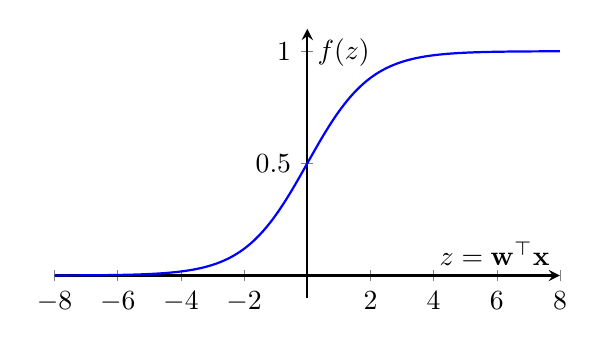
\begin{tikzpicture}
    \begin{axis}[
        axis lines = middle,
        xlabel = {$z = \mathbf{w}^\top \mathbf{x}$},
        ylabel = {$f(z)$},
        ymin = -0.1, ymax = 1.1,
        samples = 200,
        domain = -8:8,
        width=8cm,
        height=5cm,
        thick,
    ]

    \addplot[blue] {1/(1 + exp(-x))};
    \end{axis}
  \end{tikzpicture}
  \caption{Sigmoid activation function}
\end{figure}
It represents a smooth approximation of the threshold function. It is approximately linear around zero, which helps in gradient-based optimization.
However, for large positive or negative values of $z$, the function saturates (approaches 0 or 1), causing the gradient to vanish.

\subsubsection{Output Layer}
The output layer of a neural network produces the final predictions. The function used in this layer can be 
very different from the one used in hidden layers and heavily depends on the task at hand.
\\We will now analyze the activation functions used in the output layer for different tasks.
\paragraph{Binary Classification:} for binary classification tasks, only one output neuron $o(\boldsymbol{x})$ is needed.
The output activation function is usually the sigmoid activation function, which maps the output to the range (0, 1). 
It is defined as:
\[ f(\boldsymbol{x}) = \sigma(o(\boldsymbol{x})) = \frac{1}{1 + e^{-o(\boldsymbol{x})}} \]
This output can be interpreted as the probability of belonging to the positive class.
To obtain the final class label, a threshold (usually 0.5) is applied:
\[ y^* = sign(f(\boldsymbol{x}) - 0.5) \]

\paragraph{Multi-class Classification:} for multi-class classification, similar to what was done with single layer perceptron, a one vs all approach can be used.
This requires $K$ output neurons, one for each class. 
The softmax activation function is commonly used in this case, defined as:
\[ f_i(\boldsymbol{x}) = \frac{\exp(o_i(\boldsymbol{x}))}{\sum_{j=1}^{K} \exp(o_j(\boldsymbol{x}))} \quad \text{for } i = 1, 2, \ldots, K \]
Where $o_i(\boldsymbol{x})$ is the raw output score of the $i$-th output neuron.
\\This function converts the raw output scores into probabilities that sum to 1 across all classes. This is not activated element-wise, but
it is a layer-wise activation function.
The predicted class is the one with the highest probability:
\[ y^* = \arg\max_{i} f_i(\boldsymbol{x}) \] 

\paragraph{Regression:} for regression tasks, where the output is a continuous value, the decision is the value of the output neuron itself.
\[f(\boldsymbol{x}) = o(\boldsymbol{x}) \]

\subsubsection{Representational power of MLPs}
In this section we will analyze the representational power of MLPs on different tasks.
\begin{itemize}
    \item \textbf{Boolean functions:} any boolean function can be represented by a MLP with two layers of units. This can be done using CNF or DNF, but it would require
    an exponential number of hidden units in the worst case;
    \item \textbf{Continuous functions:} any bounded continuous function can be approximated arbitrarily well by a MLP with two layers of units (using sigmoid activations).
    \item \textbf{Arbitrary functions:} any function can be approximated arbitrarily well by a MLP with three layers of units (using sigmoid activations).
\end{itemize}

\subsection{Training Multi Layer Perceptrons}
Similarly to other models, MLPs are trained by minimizing a loss function on the training data. Different loss functions can be used depending on the task at hand.
\subsubsection{Loss Functions}
\paragraph{Binary Classification:}
For binary classification tasks, the binary cross-entropy loss is commonly used. It is defined as:
\[ L(y, f(\boldsymbol{x})) = - (y \log(f(\boldsymbol{x})) + (1 - y) \log(1 - f(\boldsymbol{x}))) \]
This can be interpreted as a switch function between two log-likelihoods, depending on the true label $y$. 
In fact:
\[
  \begin{cases}
  L(y, f(\boldsymbol{x})) = - \log(f(\boldsymbol{x})) & \text{if } y = 1 \\
  L(y, f(\boldsymbol{x})) = - \log(1 - f(\boldsymbol{x})) & \text{if } y = 0
  \end{cases}
\]
This is needed because, as mentioned before, $f(\boldsymbol{x})$ represents the predicted probability of belonging to the positive class. 
\\By putting the minus sign, we convert the maximization problem into a minimization one (from a likelihood to a loss).
This way, making the argument of the log function closest to 1 (correct prediction) will minimize the loss.

\paragraph{Multi-class Classification:}
For multi-class classification tasks, the cross-entropy loss is redefined for multiple classes. It is defined as:
\[ L(y, \boldsymbol{f}(\boldsymbol{x})) = - \log f_y(\boldsymbol{x}) \]
Where $f_y(\boldsymbol{x})$ is the predicted probability for the true class $y$.

\paragraph{Regression:}
For regression tasks, the mean squared error (MSE) loss is commonly used. It is defined as:
\[ L(y, f(\boldsymbol{x})) = (y - f(\boldsymbol{x}))^2 \]

\subsubsection{Stochastic Gradient Descent}
In order to train MLPs, we use Stochastic Gradient Descent (SGD) to minimize the chosen loss function. 
As example, choosing mean squared error (MSE) as loss function, we would have:
\[ E(W) = \frac{1}{2} (y - f(\boldsymbol{x}))^2 \]
Where $W$ represents all the weights in the network. Note that $\frac{1}{2}$ is added to simplify 
the derivative computation.
\\To minimize the loss function, we need to compute the gradient of the loss with respect to each weight in the network.
The relative gradient update is given by:
\[ w_{lj} = w_{lj} - \eta \frac{\partial E(W)}{\partial w_{lj}} \]
Where $\eta$ is the learning rate, $w_{lj}$ is the weight connecting neuron $j$ (source node) 
in the previous layer, to neuron $l$ (target node) in the current layer.
\\To compute the partial derivative can be quite complex when the weights are really far from the output layer, 
where we actually compute the loss (we need the output of the network to compute the loss).
\\To solve this problem, we use the Backpropagation algorithm, which efficiently computes the gradients using the chain rule of differentiation.

\subsubsection{Backpropagation}
The idea behind backpropagation is to compute the gradients layer by layer, starting from the output layer and moving backwards to the input layer.
Since each neuron's output depends on the outputs of the previous layer, which in turn depend on their own weights, we can apply the chain rule to compute the gradients.
\\\\Let's now zoom in on a single node. Suppose we want to compute the gradient of the loss function with respect to a weight $w_{lj}$ 
connecting neuron $j$ in the previous layer to neuron $l$ in the current layer.
\begin{figure}[H]
    \begin{tikzpicture}
        \node[input-node] (x1) at (0, 1.8) {};
        \node (dots) at (0, 1) {$\vdots$};
        \node[input-node, label=above right:$\phi_j$] (pred) at (0, 0) {$x_j$};
        \node (dots) at (0, -0.8) {$\vdots$};
        \node[input-node] (xm) at (0, -1.8) {};
        \node[left=0.5cm of x2] (inputs-label) {Input node $j$};

        % Node l
        \node[circle, draw, minimum size=4cm, label=above:$x_l$] (node_l) at (5, 0) {};
        \node[sum-node] (sum) at (4, 0) {\Large $\Sigma$};
        \node[activation-node, right=1.2cm of sum] (act) {
            \begin{tikzpicture}[scale=0.2] 
                \draw[blue, thick] (-1,-1) -- (0,-1) -- (0,1) -- (1,1); 
            \end{tikzpicture}
        };

        % Connection
        \draw[connection] (x1) -- (sum) node[midway, above] {};
        \draw[connection] (x2) -- (sum) node[midway, above] {$w_{lj}$};
        \draw[connection] (xm) -- (sum) node[midway, above] {};
        \draw[connection] (sum) -- (act) node[midway, above] {$a_l$};
        \draw[connection] (act) -- ++(1,0) node[right] {$\phi_l$};
    \end{tikzpicture}
\end{figure}
The chain rule gives us:
\[
\frac{\partial E(W)}{\partial w_{lj}}
= \underbrace{\frac{\partial E(W)}{\partial a_l}}_{\delta_l}
   \frac{\partial a_l}{\partial w_{lj}}
= \delta_l \, \phi_j
\]
where:
\begin{itemize}
    \item $\delta_l$ represents the error term for neuron $l$. 
    Represents how much the output of neuron $l$ contributes to the final error;
    \item $\phi_j$ is the output of neuron $j$ in the previous layer. It is one of the inputs of the node $l$;
    \item $\frac{\partial a_l}{\partial w_{lj}}$ is the input $\phi_j$. Since $a_l = \sum_{i} w_{li} \phi_i$,
    if we derive with respect to $w_{lj}$ all terms are constant except for the one with $i = j$, which gives $\phi_j$.
\end{itemize}
The final update rule for weight $w_{lj}$ is simply the error term $\delta_l$ multiplied by the input $\phi_j$ coming from the previous layer.
\\The computation of $\delta_l$ depends on whether neuron $l$ is in the output layer or in a hidden layer. We will analyze both cases.

\paragraph{Output layers:}
Since neuron $l$ is in the output layer, we can directly compute the derivative 
of the loss function with respect to the output of the network. Considering the MSE loss function, we have:
\[\delta_{o} = \frac{\partial E(W)}{\partial a_{o}} = \frac{\partial \frac{1}{2} (y - f(\boldsymbol{x}))^2}{\partial a_{o}} \]
Since we do not apply a non-linear activation function in the output layer for regression tasks, we have that $f(\boldsymbol{x}) = a_{o}$, so:
\[ = \frac{\partial \frac{1}{2} (y - a_0)^2}{\partial a_{o}} = -(y - a_{o}) \]

\paragraph{Hidden layers:}
Here the node $l$ is in a hidden layer. Since we compute $\delta_l$ using the chain rule, 
we need to consider the contributions from the neurons in the next layer.
\[\delta_{l} = \frac{\partial E(W)}{\partial a_{l}} = \sum_{k \in \text{children}(l)} \frac{\partial E(W)}{\partial a_{k}} \frac{\partial a_{k}}{\partial a_{l}} \]
Where $k$ are the neurons in the next layer connected to neuron $l$. Intuitively, we are computing the contribution of neuron $l$ to the final error, by considering all the paths from $l$ to the output layer.
\\The term $\frac{\partial E(W)}{\partial a_{k}}$ is simply $\delta_k$, already computed in the next layer. We derive that:
\[\delta_{l} = \sum_{k \in \text{children}(l)} \delta_k \frac{\partial a_{k}}{\partial a_{l}} \]
Remembering that $a_k = \sum_{m} w_{km} \phi_m$, where $\phi_m$ is the output of neuron $m$ in the previous layer, we have that:
\[\frac{\partial a_{k}}{\partial a_{l}} = \frac{\partial a_{k}}{\partial \phi_{l}} \frac{\partial \phi_{l}}{\partial a_{l}}\]
The first term is simply the weight $w_{kl}$. The second term is the derivative of the activation function $\sigma(\cdot)$ used in neuron $l$.
Putting everything together, we have:
\[\delta_{l} = \sum_{k \in \text{children}(l)} \delta_k w_{kl} \sigma(a_{l})(1 - \sigma(a_{l})) \]
Where we used the derivative of the sigmoid activation function $(\frac{\partial \sigma(x)}{\partial x} = \sigma(x)(1 - \sigma(x)))$.

\subsection{Modular Structure of Neural Networks}
Neural networks can be seen as a combination of different modules, each with a specific function. Each of these modules has an interface to communicate with other modules.
Each layer $j$ takes as input  $\phi_{j-1}$ and it's weights $W_j$, and produces as output $\phi_{j} = F(\phi_{j-1}, W_j)$. Once we get to the output layer, we can compute the loss function and the gradients using backpropagation.
\[\frac{\partial E(W)}{\partial W_j} = \frac{\partial E(W)}{\partial \phi_j} \frac{\partial \phi_j}{\partial W_j}  = \frac{\partial E(W)}{\partial \phi_j} \frac{\partial F_j(\phi_{j-1}, W_j)}{\partial W_j}\]
Each layer computes:
\[ \frac{\partial E(W)}{\partial \phi_{j-1}} = \frac{\partial E(W)}{\partial \phi_j} \frac{\partial \phi_j}{\partial \phi_{j-1}} = \frac{\partial E(W)}{\partial \phi_j} \frac{\partial F_j(\phi_{j-1}, W_j)}{\partial \phi_{j-1}} \]
Each module must be able to compute:
\begin{itemize}
    \item the derivative of its output with respect to its weights:
    \[ \frac{\partial \phi_j}{\partial W_j} = \frac{\partial F_j(\phi_{j-1}, W_j)}{\partial W_j} \]
    \item the derivative of its output with respect to its input:
    \[ \frac{\partial \phi_j}{\partial \phi_{j-1}} = \frac{\partial F_j(\phi_{j-1}, W_j)}{\partial \phi_{j-1}} \]
\end{itemize}

\subsection{Remarks on Training Neural Networks}
The error surface of neural networks is non-convex. This implies that there can be multiple local minima and backpropagation is only guaranteed to find a local minimum.
There are many techniques to improve the training of neural networks, that we will cover later in this section.
\subsubsection{Stopping Criteria}
Overtraining the network can increase the possibility of overfitting the training data. When the network is initialized, the weights are set to small random values. In this phase, we have a very simple surface, which is easy to optimize.
\\As the weights are updated, the surface becomes more complex, and the risk of overfitting increases.
To avoid this, a separate validation set is used to monitor the performance of the network during training. When the performance on the validation set starts to degrade, training is stopped.
\subsubsection{Vanishing gradients}
A common problem when training deep neural networks is the vanishing gradient problem. During backpropagation, at each step the 
gradient is multiplied by the derivative of the activation function (sigmoid in our case). 
Since the saturated regions of the sigmoid have very small derivatives, the gradients can become very small as they are propagated back through the layers.
A few simple suggestions to mitigate this problem are:
\begin{itemize}
    \item \textbf{Weight initialization:} initialize the weights to small random values;
    \item \textbf{Normalization:} normalize the input data to have zero mean and unit variance ($X' = \frac{X - \mu_x}{\sigma_x}$)
\end{itemize}
Other tricks of the trade will be covered in the next paragraph.
\paragraph{Activations functions:}
Since the main problem generating vanishing gradients is the use of the sigmoid activation function, a new activation function has been proposed: the ReLU (Rectified Linear Unit).
It is defined as:
\[ f(x) = \max(0, \boldsymbol{w}^T \boldsymbol{x}) \]
Where $\boldsymbol{w}^T \boldsymbol{x}$ represents the weighted sum of inputs to the neuron.
\begin{center}
\begin{tikzpicture}
\begin{axis}[
    axis lines = middle,
    xlabel = {$z = \mathbf{w}^\top \mathbf{x}$},
    ylabel = {$f(z)$},
    ymin = -1, ymax = 6,
    samples = 200,
    domain = -4:4,
    width=10cm,
    height=6cm,
    thick,
]
\addplot[blue] {(x > 0) * x};
\end{axis}
\end{tikzpicture}
\end{center}
The ReLU activation function does not saturate for positive values, and its derivative is constant (1) in that region. This helps to mitigate the vanishing gradient problem.

\paragraph{Regularization:}
Two common regularization techniques used in training neural networks are:
\begin{itemize}
  \item \textbf{2-norm regularization:} adding a penalty term to the loss function proportional to the euclidean norm of the weights.
  \[ J(W) = E(W) + \lambda ||W||_2 \]
  In essence, this encourages less relevant weights to be small, reducing overfitting.
  \item \textbf{1-norm regularization:} adding a penalty term to the loss function proportional to the absolute value of the weights.
  This encourages less relevant weights to be exactly zero.
  \[ J(W) = E(W) + \lambda |W| \]
\end{itemize}

\paragraph{Initialization:}
Random initialization of weights is crucial for braking symmetry between neurons. If all weights are initialized to the same value, all neurons in a layer will learn the same features.
A common approach is to initialize weights randomly, from a uniform distribution in the range:
\[ W_{ij} \sim U\left(-\frac{\sqrt{6}}{\sqrt{n + m}}, \frac{\sqrt{6}}{\sqrt{n + m}}\right) \]
Where $n$ is the number of input units and $m$ is the number of output units.

\paragraph{Gradient descent:}
\begin{itemize}
  \item \textbf{Batch Gradient Descent:} updates weights after seeing the entire training set. This can be computationally expensive for large datasets;
  \item \textbf{Stochastic Gradient Descent:} updates weights after seeing each training example. The final objective function is noisy and may be different from the true objective;
  \item \textbf{Mini-batch Gradient Descent:} updates weights after seeing a small batch of training examples. The size of the batch is usually associated with the hardware capabilities (e.g., GPU memory). 
\end{itemize}

\paragraph{Momentum:}
Momentum is a technique used to accelerate gradient descent and escape local minima. The idea is to update the weights using
a combination of the current gradient and the previous updates, similar to a ball rolling down a hill.
The update rule with momentum is given by:
\[v_{ji}^\text{(new)} = \alpha v_{ji}^\text{(old)} - \eta \frac{\partial E(W)}{\partial w_{ji}}\]
\[w_{ji}^\text{(new)} = w_{ji}^\text{(old)} + v_{ji}^\text{(new)}\]
Where:
\begin{itemize}
    \item $\alpha$ is the momentum coefficient. $0 \le \alpha < 1$
    \item $v_{ji}$ is the velocity term for weight $w_{ji}$;
\end{itemize}

\paragraph{Adaptive Learning Rates:}
Adaptive learning rate methods adjust the learning rate during training based on the progress made.
Some popular methods are:
\begin{itemize}
    \item \textbf{Decreasing learning rate:} gradually decrease the learning rate over time.
    \[\eta_t = \begin{cases}
    (1 - \frac{t}{\tau})\eta_0 + \frac{t}{\tau} \eta_{\text{min}}  & \text{if } t < \tau \\
    \eta_{\text{min}} & \text{if } t \ge \tau
    \end{cases}
    \]
    The idea is to start with a high learning rate to explore the error surface, and then decrease to avoid oscillations around minima.
    The learning rate is decreased linearly from $\eta_0$ to $\eta_{\text{min}}$ over $\tau$ iterations. After that, it remains constant at $\eta_{\text{min}}$;
    \item \textbf{AdaGrad:} adapts the learning rate for each weight based on the historical gradients.
    \[ r_{ji}^\text{(new)} = r_{ji}^\text{(old)} + \left(\frac{\partial E(W)}{\partial w_{ji}}\right)^2 \]
    \[ w_{ji}^\text{(new)} = w_{ji}^\text{(old)} - \frac{\eta}{\sqrt{r_{ji}^\text{(new)}}} \frac{\partial E(W)}{\partial w_{ji}} \]
    Where $r_{ji}$ accumulates the squared gradients for weight $w_{ji}$. This results in smaller updates for weights with large gradients (steep directions) and larger updates for weights with small gradients (flat directions);
    This has a drawback: the accumulated squared gradients can grow indefinitely.
    \item \textbf{RMSProp:} addresses the drawback of AdaGrad by using an exponentially decaying average of squared gradients.
    \[ r_{ji}^\text{(new)} = \rho r_{ji}^\text{(old)} + (1 - \rho) \left(\frac{\partial E(W)}{\partial w_{ji}}\right)^2 \]
    \[ w_{ji}^\text{(new)} = w_{ji}^\text{(old)} - \frac{\eta}{\sqrt{r_{ji}^\text{(new)} + \epsilon}} \frac{\partial E(W)}{\partial w_{ji}} \]
    Where $\rho$ allows to exponentially decay the influence of past gradients.
\end{itemize}
\paragraph{Batch Normalization:}
To mitigate the problem of internal covariate shift, batch normalization is used. It normalizes the input of each activation function on its mini-batch.
\[ \hat{x_i} = \frac{x_i - \mu_B}{\sigma_B}\]
Where $\mu_B$ and $\sigma_B$ are the mean and standard deviation of the mini-batch $B$, $x$ is the activation of an arbitrary layer.
This normalization helps to stabilize the learning process and allows for higher learning rates.
\subsection{Popular architectures}
Different architectures of neural networks have been proposed to tackle specific problems. In this section we will briefly describe some of the most popular ones.
\subsubsection*{Autoencoders}
Autoencoders are a type of neural network used for unsupervised learning (learning with no labelled data). They consist of an
encoder, that maps the input data to a lower-dimensional latent space, and a decoder, that reconstructs the input data from the latent representation.
This is useful for dimensionality reduction, feature learning, and data compression.
\subsubsection*{Convolutional Neural Networks (CNNs)}
Convolutional Neural Networks (CNNs) are specialized neural networks designed for processing grid-like data, such as images. 
They use convolutional filters to extract local features from the input data. Pooling layers are used to compose higher-level features from lower-level ones.
After several convolutional and pooling layers, fully connected layers are used to perform the final classification.
\subsubsection*{Generative Adversarial Networks (GANs)}
Generative Adversarial Networks (GANs) learns to generate items from random noise. 
They consist of two neural networks: a generator, that generates new data, and a discriminator, that tries to distinguish between real and generated data.
The two networks are trained simultaneously, with no supervision needed.
\subsubsection*{Transformers}
Use attention mechanisms to learn input words encodings, that depends on the context of the sentence.
They can also learn output words encodings, that depends on the context of the already generated words and on the input sentence.
\subsubsection*{Graph Neural Networks (GNNs)}
Allow to learn from graph-structured data. Allow to propagate information from a node to its neighbors, learning a representation that takes into account the graph structure.
